\problemname{Low Effort League}

The teams in your local rugby league aren't particularly good, but they make up
for it in enthusiasm. We are going to organise a single-elimination knockout
tournament between them, where the $2^n$ teams play $n$ rounds. In each round,
the $2i+1$th remaining team pairs up with the $2i+2$th team and one or the
other team is eliminated.

\begin{figure}[h!]
  \centering
  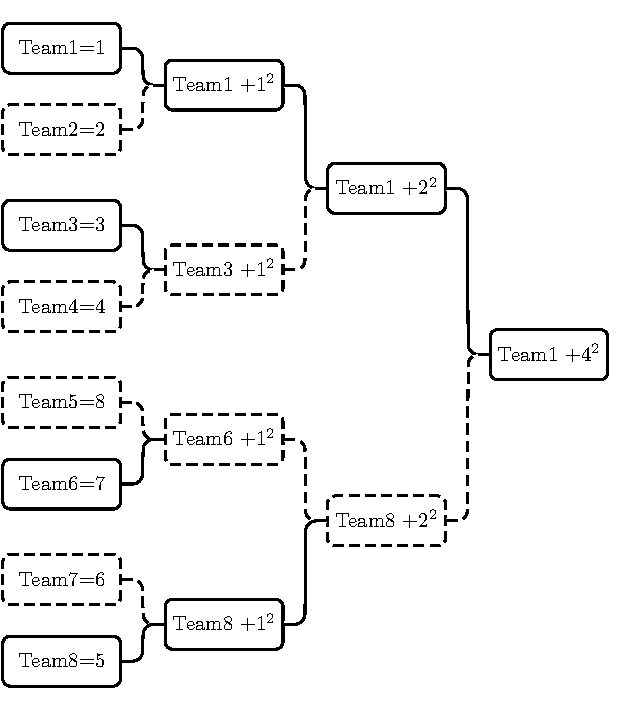
\includegraphics[width=0.35\textwidth]{sample2}
 \label{fig:loweffortleague}
\end{figure}

Each team has a scalar skill level. In the normal course of things, a team with
higher skill level will always beat a team with lower skill level. However,
training plays a part too: if one team studies another, learns its techniques,
and trains against them, it can win.

The number of hours a team with skill $a$ must train to beat a team with skill
$b$ (where $a \le b$) is $|b-a|^2$. This training only affects that one game
(it does not transfer to other teams).

You would quite like your favourite team to win the tournament. If you take
complete control over how every team trains, you can always make this happen.
What is the minimum number of hours needed, in total across all teams, in order
for your team (team $1$) to win?

\section*{Input}

The input consists of:
\begin{itemize}
  \item one line containing the integer $r$ ($1 \le r \le 14 $), the number of
        rounds in the tournament.
  \item one line with $2\textsuperscript{r}$ integers $s_1 \ldots
        s_2\textsuperscript{s}$ ($0 \leq s_i \leq 10^6$ for each $i$), where $s_i$
        is the skill level of the $i$th team.
\end{itemize}

\section*{Output}

Output the smallest number of hours needed for team $1$ to win the tournament.
